    
    
    
    

    

    \hypertarget{caractuxe8res-accentuuxe9s}{%
\section{Caractères accentués}\label{caractuxe8res-accentuuxe9s}}

    Ce complément expose quelques bases concernant les caractères accentués,
et notamment les précautions à prendre pour pouvoir en insérer dans un
programme Python. Nous allons voir que cette question, assez scabreuse,
dépasse très largement le cadre de Python.

    \hypertarget{compluxe9ment---niveau-basique}{%
\subsection{Complément - niveau
basique}\label{compluxe9ment---niveau-basique}}

    \hypertarget{un-caractuxe8re-nest-pas-un-octet}{%
\subparagraph{Un caractère n'est pas un
octet}\label{un-caractuxe8re-nest-pas-un-octet}}

    Avec Unicode, on a cassé le modèle \emph{un caractère} == \emph{un
octet}. Aussi en Python 3, lorsqu'il s'agit de manipuler des données
provenant de diverses sources de données~:

\begin{itemize}
\tightlist
\item
  le type \texttt{byte} est approprié si vous voulez charger en mémoire
  les données binaires brutes, sous forme d'octets donc~;
\item
  le type \texttt{str} est approprié pour représenter une chaîne de
  caractères - qui, à nouveau ne sont pas forcément des octets~;
\item
  on passe de l'un à l'autre de ces types par des opérations d'encodage
  et décodage, comme illustré ci-dessous~;
\item
  et pour \textbf{toutes} les opérations d'encodage et décodage, il est
  nécessaire de connaître l'encodage utilisé.
\end{itemize}

    \begin{figure}
\centering
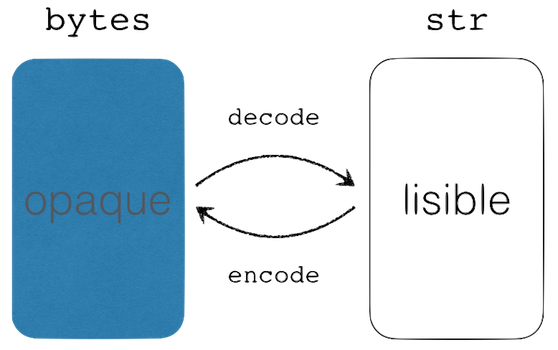
\includegraphics{media/str-bytes.png}
\caption{les types bytes et str}
\end{figure}

    On peut appeler les méthodes \texttt{encode} et \texttt{decode} sans
préciser l'encodage (dans ce cas Python choisit l'encodage par défaut
sur votre système). Cela dit, il est de loin préférable d'être explicite
et de choisir son encodage. En cas de doute, il est recommandé de
\textbf{spécifier explicitement} \texttt{utf-8}, qui se généralise au
détriment d'encodages anciens comme \texttt{cp1242} (Windows) et
\texttt{iso8859-*}, que de laisser le système hôte choisir pour vous.

    \hypertarget{utilisation-des-accents-et-autres-cuxe9dilles}{%
\subparagraph{Utilisation des accents et autres
cédilles}\label{utilisation-des-accents-et-autres-cuxe9dilles}}

    Python 3 supporte Unicode par défaut. Vous pouvez donc, maintenant,
utiliser sans aucun risque des accents ou des cédilles dans vos chaînes
de caractères. Il faut cependant faire attention à deux choses~:

\begin{itemize}
\tightlist
\item
  Python supporte Unicode, donc tous les caractères du monde, mais les
  ordinateurs n'ont pas forcément les polices de caractères nécessaires
  pour afficher ces caractères~;
\item
  Python permet d'utiliser des caractères Unicode pour les noms de
  variables, mais nous vous recommandons dans toute la mesure du
  possible d'écrire votre code en anglais, comme c'est le cas pour la
  quasi-totalité du code que vous serez amenés à utiliser sous forme de
  bibliothèques. Ceci est particulièrement important pour les noms de
  lignes et de colonnes dans un dataset afin de faciliter les transferts
  entre logiciels, la majorité des logiciels n'acceptant pas les accents
  et cédilles dans les noms de variables.
\end{itemize}

Ainsi, il faut bien distinguer les chaînes de caractères qui doivent par
nature être adaptées au langage des utilisateurs du programme, et le
code source qui lui est destiné aux programmeurs et qui doit donc éviter
d'utiliser autre chose que de l'anglais.

    \hypertarget{compluxe9ment---niveau-intermuxe9diaire}{%
\subsection{Complément - niveau
intermédiaire}\label{compluxe9ment---niveau-intermuxe9diaire}}

    \hypertarget{ouxf9-peut-on-mettre-des-accents}{%
\subsubsection{Où peut-on mettre des
accents~?}\label{ouxf9-peut-on-mettre-des-accents}}

    Cela étant dit, si vous devez vraiment mettre des accents dans vos
sources, voici ce qu'il faut savoir.

    \hypertarget{noms-de-variables}{%
\paragraph{Noms de variables}\label{noms-de-variables}}

    \begin{itemize}
\tightlist
\item
  S'il n'était \textbf{pas possible en Python 2} d'utiliser un caractère
  accentué dans un \textbf{nom de variable} (ou d'un identificateur au
  sens large), cela est à présent \textbf{permis en Python 3}~:
\end{itemize}

    \begin{Verbatim}[commandchars=\\\{\},frame=single,framerule=0.3mm,rulecolor=\color{cellframecolor}]
{\color{incolor}In [{\color{incolor}1}]:} \PY{c+c1}{\PYZsh{} pas recommandé, mais autorisé par le langage}
        \PY{n}{nb\PYZus{}élèves} \PY{o}{=} \PY{l+m+mi}{12}
\end{Verbatim}


    \begin{itemize}
\tightlist
\item
  On peut même utiliser des symboles, comme par exemple
\end{itemize}

    \begin{Verbatim}[commandchars=\\\{\},frame=single,framerule=0.3mm,rulecolor=\color{cellframecolor}]
{\color{incolor}In [{\color{incolor}2}]:} \PY{k+kn}{from} \PY{n+nn}{math} \PY{k}{import} \PY{n}{cos}\PY{p}{,} \PY{n}{pi} \PY{k}{as} \PY{n}{𝞟}
        \PY{n}{θ} \PY{o}{=} \PY{n}{𝞟} \PY{o}{/} \PY{l+m+mi}{4}
        \PY{n}{cos}\PY{p}{(}\PY{n}{θ}\PY{p}{)}
\end{Verbatim}


\begin{Verbatim}[commandchars=\\\{\},frame=single,framerule=0.3mm,rulecolor=\color{cellframecolor}]
{\color{outcolor}Out[{\color{outcolor}2}]:} 0.7071067811865476
\end{Verbatim}
            
    \begin{itemize}
\tightlist
\item
  Je vous recommande toutefois de \textbf{ne pas utiliser} cette
  possibilité, si vous n'êtes pas extrêmement familier avec les
  caractères Unicode.
\end{itemize}

    \begin{itemize}
\tightlist
\item
  Enfin, pour être exhaustif, sachez que seule une partie des caractères
  Unicode sont autorisés dans ce cadre, c'est heureux parce que les
  caractères comme, par exemple,
  \href{http://www.fileformat.info/info/unicode/char/a0/index.htm}{l'espace
  non-sécable} pourraient, s'ils étaient autorisés, être la cause de
  milliers d'heures de debugging à frustration garantie :)
\end{itemize}

Pour les curieux, vous pouvez en savoir plus
\href{https://docs.python.org/3/reference/lexical_analysis.html\#identifiers}{à
cet endroit de la documentation officielle (en anglais)}.

    \hypertarget{chauxeenes-de-caractuxe8res}{%
\paragraph{Chaînes de caractères}\label{chauxeenes-de-caractuxe8res}}

    \begin{itemize}
\item
  Vous pouvez naturellement mettre des accents dans les chaînes de
  caractères. Cela dit, les données manipulées par un programme
  proviennent pour l'essentiel de sources externes, comme une base de
  données ou un formulaire Web, et donc le plus souvent pas directement
  du code source. Les chaînes de caractères présentes dans du vrai code
  sont bien souvent limitées à des messages de logging, et le plus
  souvent d'ailleurs en anglais, donc sans accent.
\item
  Lorsque votre programme doit interagir avec les utilisateurs et qu'il
  doit donc parler leur langue, c'est une bonne pratique de créer un
  fichier spécifique, que l'on appelle fichier de ressources, qui
  contient toutes les chaînes de caractères spécifiques à une langue.
  Ainsi, la traduction de votre programme consistera à simplement
  traduire ce fichier de ressources.
\end{itemize}

    \begin{Shaded}
\begin{Highlighting}[frame=lines,framerule=0.6mm,rulecolor=\color{asisframecolor}]
\NormalTok{message }\OperatorTok{=} \StringTok{"on peut mettre un caractère accentué dans une chaîne"}
\end{Highlighting}
\end{Shaded}

    \hypertarget{commentaires}{%
\paragraph{Commentaires}\label{commentaires}}

    \begin{itemize}
\tightlist
\item
  Enfin on peut aussi bien sûr mettre dans les commentaires n'importe
  quel caractère Unicode, et donc notamment des caractères accentués si
  on choisit malgré tout d'écrire le code en français.
\end{itemize}

    \begin{Shaded}
\begin{Highlighting}[frame=lines,framerule=0.6mm,rulecolor=\color{asisframecolor}]
\CommentTok{# on peut mettre un caractère accentué dans un commentaire}
\CommentTok{# ainsi que cos(Θ), ∀x ∈ ∫f(t)dt vous voyez l'idée générale}
\end{Highlighting}
\end{Shaded}

    \hypertarget{quest-ce-quun-encodage}{%
\subsubsection{Qu'est-ce qu'un
encodage~?}\label{quest-ce-quun-encodage}}

    Comme vous le savez, la mémoire - ou le disque - d'un ordinateur ne
permet que de stocker des représentations binaires. Il n'y a donc pas de
façon ``naturelle'' de représenter un caractère comme `A', un guillemet
ou un point-virgule.

On utilise pour cela un encodage, par exemple le code \texttt{US-ASCII}
- http://www.asciitable.com/ - stipule, pour faire simple, qu'un `A' est
représenté par l'octet 65 qui s'écrit en binaire 01000001. Il se trouve
qu'il existe plusieurs encodages, bien sûr incompatibles, selon les
systèmes et les langues. Vous trouverez plus de détails ci-dessous.

Le point important est que pour pouvoir ouvrir un fichier
``proprement'', il faut bien entendu disposer du \textbf{contenu} du
fichier, mais il faut aussi connaître l'\textbf{encodage} qui a été
utilisé pour l'écrire.

    \hypertarget{pruxe9cautions-uxe0-prendre-pour-lencodage-de-votre-code-source}{%
\subsubsection{Précautions à prendre pour l'encodage de votre code
source}\label{pruxe9cautions-uxe0-prendre-pour-lencodage-de-votre-code-source}}

    L'encodage ne concerne pas simplement les objets chaîne de caractères,
mais également votre code source. \textbf{Python 3} considère que votre
code source utilise \textbf{par défaut l'encodage \texttt{UTF-8}}. Nous
vous conseillons de conserver cet encodage qui est celui qui vous
offrira le plus de flexibilité.

    Vous pouvez malgré tout changer l'encodage \textbf{de votre code source}
en faisant figurer dans vos fichiers, \textbf{en première ou deuxième
ligne}, une déclaration comme ceci~:

\begin{Shaded}
\begin{Highlighting}[frame=lines,framerule=0.6mm,rulecolor=\color{asisframecolor}]
\CommentTok{# -*- coding: <nom_de_l_encodage> -*-}
\end{Highlighting}
\end{Shaded}

ou plus simplement, comme ceci~:

\begin{Shaded}
\begin{Highlighting}[frame=lines,framerule=0.6mm,rulecolor=\color{asisframecolor}]
\CommentTok{# coding: <nom_de_l_encodage>}
\end{Highlighting}
\end{Shaded}

Notons que la première option est également interprétée par l'éditeur de
texte \emph{Emacs} pour utiliser le même encodage. En dehors de
l'utilisation d'Emacs, la deuxième option, plus simple et donc plus
pythonique, est à préférer.

    Le nom \textbf{\texttt{UTF-8}} fait référence à \textbf{Unicode} (ou
pour être précis, à l'encodage le plus répandu parmi ceux qui sont
définis dans la norme Unicode, comme nous le verrons plus bas). Sur
certains systèmes plus anciens vous pourrez être amenés à utiliser un
autre encodage. Pour déterminer la valeur à utiliser dans votre cas
précis vous pouvez faire dans l'interpréteur interactif~:

    \begin{Shaded}
\begin{Highlighting}[frame=lines,framerule=0.6mm,rulecolor=\color{asisframecolor}]
\CommentTok{# ceci doit être exécuté sur votre machine}
\ImportTok{import}\NormalTok{ sys}
\BuiltInTok{print}\NormalTok{(sys.getdefaultencoding())}
\end{Highlighting}
\end{Shaded}

    Par exemple avec d'anciennes versions de Windows (en principe de plus en
plus rares) vous pouvez être amenés à écrire~:

    \begin{Shaded}
\begin{Highlighting}[frame=lines,framerule=0.6mm,rulecolor=\color{asisframecolor}]
\CommentTok{# coding: cp1252}
\end{Highlighting}
\end{Shaded}

    La syntaxe de la ligne \texttt{coding} est précisée dans
\href{https://docs.python.org/3/reference/lexical_analysis.html\#encoding-declarations}{cette
documentation} et dans le
\href{https://www.python.org/dev/peps/pep-0263/}{PEP 263}.

    \hypertarget{le-grand-malentendu}{%
\subsubsection{Le grand malentendu}\label{le-grand-malentendu}}

    Si je vous envoie un fichier contenant du français encodé avec, disons,
\texttt{ISO/IEC\ 8859-15} (\texttt{Latin-9}) --
http://en.wikipedia.org/wiki/ISO/IEC\_8859-15 -- vous pouvez voir dans
la table qu'un caractère `€' va être matérialisé dans mon fichier par un
octet `0xA4', soit 164.

Imaginez maintenant que vous essayez d'ouvrir ce même fichier depuis un
vieil ordinateur Windows configuré pour le français. Si on ne lui donne
aucune indication sur l'encodage, le programme qui va lire ce fichier
sur Windows va utiliser l'encodage par défaut du système, c'est-à-dire
\texttt{CP1252} -- http://en.wikipedia.org/wiki/Windows-1252. Comme vous
le voyez dans cette table, l'octet `0xA4' correspond au caractère

\includegraphics{media/currency-sign.png} et c'est ça que vous allez
voir à la place de €.

Contrairement à ce qu'on pourrait espérer, ce type de problème ne peut
pas se régler en ajoutant une balise
\texttt{\#\ coding:\ \textless{}nom\_de\_l\_encodage\textgreater{}}, qui
n'agit que sur l'encodage utilisé \emph{pour lire le fichier source en
question} (celui qui contient la balise).

Pour régler correctement ce type de problème, il vous faut préciser
explicitement l'encodage à utiliser pour décoder le fichier. Et donc
avoir un moyen fiable de déterminer cet encodage; ce qui n'est pas
toujours aisé d'ailleurs, mais c'est une autre discussion
malheureusement. Ce qui signifie que pour être totalement propre, il
faut pouvoir préciser explicitement le paramètre \texttt{encoding} à
l'appel de toutes les méthodes qui sont susceptibles d'en avoir besoin.

    \hypertarget{pourquoi-uxe7a-marche-en-local}{%
\subsubsection{Pourquoi ça marche en
local~?}\label{pourquoi-uxe7a-marche-en-local}}

    Lorsque le producteur (le programme qui écrit le fichier) et le
consommateur (le programme qui le lit) tournent dans le même ordinateur,
tout fonctionne bien - en général - parce que les deux programmes se
ramènent à l'encodage défini comme l'encodage par défaut.

Il y a toutefois une limite, si vous utilisez un Linux configuré de
manière minimale, il se peut qu'il utilise par défaut l'encodage
\texttt{US-ASCII} - voir plus bas - qui étant très ancien ne ``connaît''
pas un simple é, ni a fortiori €. Pour écrire du français, il faut donc
au minimum que l'encodage par défaut de votre ordinateur contienne les
caractères français, comme par exemple~:

\begin{itemize}
\tightlist
\item
  \texttt{ISO\ 8859-1} (\texttt{Latin-1})
\item
  \texttt{ISO\ 8859-15} (\texttt{Latin-9})
\item
  \texttt{UTF-8}
\item
  \texttt{CP1252}
\end{itemize}

À nouveau dans cette liste, il faut clairement préférer UTF-8 lorsque
c'est possible.

    \hypertarget{un-peu-dhistoire-sur-les-encodages}{%
\subsubsection{Un peu d'histoire sur les
encodages}\label{un-peu-dhistoire-sur-les-encodages}}

    \hypertarget{le-code-us-ascii}{%
\subparagraph{\texorpdfstring{Le code
\texttt{US-ASCII}}{Le code US-ASCII}}\label{le-code-us-ascii}}

    Jusque dans les années 1980, les ordinateurs ne parlaient pour
l'essentiel que l'anglais. La première vague de standardisation avait
créé l'encodage dit \texttt{ASCII}, ou encore \texttt{US-ASCII} - voir
par exemple http://www.asciitable.com, ou en version longue
http://en.wikipedia.org/wiki/ASCII.

Le code \texttt{US-ASCII} s'étend sur 128 valeurs, soit 7 bits, mais est
le plus souvent implémenté sur un octet pour préserver l'alignement, le
dernier bit pouvant être utilisé par exemple pour ajouter un code
correcteur d'erreur - ce qui à l'époque des modems n'était pas superflu.
Bref, la pratique courante était alors de manipuler une chaîne de
caractères comme un tableau d'octets.

    \hypertarget{les-encodages-iso8859--latin}{%
\subparagraph{\texorpdfstring{Les encodages \texttt{ISO8859-*}
(\texttt{Latin*})}{Les encodages ISO8859-* (Latin*)}}\label{les-encodages-iso8859--latin}}

    Dans les années 1990, pour satisfaire les besoins des pays européens,
ont été définis plusieurs encodages alternatifs, connus sous le nom de
\href{http://en.wikipedia.org/wiki/ISO/IEC_8859}{\texttt{ISO/IEC\ 8859-*}},
nommés aussi \texttt{Latin-*}. Idéalement, on aurait pu et
\textbf{certainement dû} définir un seul encodage pour représenter tous
les nouveaux caractères, mais entre toutes les langues européennes, le
nombre de caractères à ajouter était substantiel, et cet encodage unifié
aurait largement dépassé 256 caractères différents, il n'aurait donc
\textbf{pas été possible} de tout faire tenir sur un octet.

On a préféré préserver la ``bonne propriété'' du modèle \emph{un
caractère} == \emph{un octet}, ceci afin de préserver le code existant
qui aurait sinon dû être retouché ou réécrit.

Dès lors il n'y avait pas d'autre choix que de définir
\textbf{plusieurs} encodages distincts, par exemple, pour le français on
a utilisé à l'époque
\href{http://en.wikipedia.org/wiki/ISO/IEC_8859-1}{\texttt{ISO/IEC\ 8859-1}
(\texttt{Latin-1})}, pour le russe
\href{http://en.wikipedia.org/wiki/ISO/IEC_8859-5}{\texttt{ISO/IEC\ 5589-5}
(\texttt{Latin/Cyrillic})}.

À ce stade, le ver était dans le fruit. Depuis cette époque pour ouvrir
un fichier il faut connaître son encodage.

    \hypertarget{unicode}{%
\subparagraph{Unicode}\label{unicode}}

    Lorsque l'on a ensuite cherché à manipuler aussi les langues asiatiques,
il a de toute façon fallu définir de nouveaux encodages beaucoup plus
larges. C'est ce qui a été fait par le standard
\href{http://en.wikipedia.org/wiki/Unicode}{Unicode} qui définit 3
nouveaux encodages~:

\begin{itemize}
\tightlist
\item
  \href{http://en.wikipedia.org/wiki/UTF-8}{\texttt{UTF-8}} : un
  encodage à taille variable, à base d'octets, qui maximise la
  compatibilité avec US-ASCII~;
\item
  \href{http://en.wikipedia.org/wiki/UTF-16}{\texttt{UTF-16}} : un
  encodage à taille variable, à base de mots de 16 bits~;
\item
  \href{http://en.wikipedia.org/wiki/UTF-32}{\texttt{UTF-32}} : un
  encodage à taille fixe, à base de mots de 32 bits~;
\end{itemize}

Ces 3 standards couvrent le même jeu de caractères (113 021 tout de même
dans la dernière version). Parmi ceux-ci le plus utilisé est
certainement \texttt{UTF-8}. Un texte ne contenant que des caractères du
code \texttt{US-ASCII} initial peut être lu avec l'encodage
\texttt{UTF-8}.

Pour être enfin tout à fait exhaustif, si on sait qu'un fichier est au
format Unicode, on peut déterminer quel est l'encodage qu'il utilise, en
se basant sur les 4 premiers octets du document. Ainsi dans ce cas
particulier (lorsqu'on est sûr qu'un document utilise un des trois
encodages Unicode) il n'est plus nécessaire de connaître son encodage de
manière ``externe''.


    % Add a bibliography block to the postdoc
    
    
    
